% Text Recognition of Ancient Greek "Squeezes"
% Compile with: lualatex report.tex  (run twice for references)
\documentclass[11pt]{article}

\usepackage{fontspec}
\defaultfontfeatures{Ligatures=TeX}
\setmainfont{Latin Modern Roman}
\setmonofont{Latin Modern Mono}[Scale=MatchLowercase,RawFeature={-tlig}]
\usepackage[a4paper,margin=1.0in]{geometry}
\usepackage{amsmath}
\usepackage{amssymb}
\usepackage{graphicx}
\usepackage{booktabs}
\usepackage{array}
\usepackage{caption}
\usepackage{subcaption}
\usepackage{float}
\usepackage{enumitem}
\usepackage{xcolor}
\usepackage{setspace}
\usepackage{tikz}
\usetikzlibrary{positioning,arrows.meta,fit,backgrounds,calc}
\usepackage[protrusion=true,expansion=true,final]{microtype}
\usepackage{placeins}
\usepackage[hidelinks,colorlinks=true,linkcolor=black,citecolor=black,urlcolor=blue!55!black]{hyperref}

\setstretch{1.12}
\setlength{\parskip}{0.35em plus 0.1em}
\captionsetup{font=small,labelfont=bf}
\captionsetup[sub]{font=footnotesize}
\setlist{itemsep=2.5pt,topsep=3pt,parsep=0pt,leftmargin=1.6em}
\setlength{\tabcolsep}{5pt}
\setlength{\emergencystretch}{2em}
\renewcommand{\topfraction}{0.92}
\renewcommand{\bottomfraction}{0.7}
\renewcommand{\textfraction}{0.06}
\renewcommand{\floatpagefraction}{0.8}

\definecolor{accent}{HTML}{1F4E79}
\definecolor{baseblue}{HTML}{D6E4F0}
\definecolor{addgold}{HTML}{F2C14E}
\definecolor{addgoldbg}{HTML}{FBEFD3}
\newcommand{\cer}{\mbox{CER}}
\newcommand{\squeeze}{\textit{squeeze}}
\newcommand{\model}{\texttt{SqueezeTrOCR}}
\newcommand{\charpost}{\texttt{charpost}}
\newcommand{\maybeinclude}[2][]{%
  \IfFileExists{#2}{\includegraphics[#1]{#2}}{%
    \fbox{\parbox{0.86\linewidth}{Missing figure: \texttt{#2}}}}}

\tikzset{
  basebox/.style={draw=accent!70,fill=baseblue,rounded corners=2pt,align=center,
    font=\footnotesize,inner sep=4pt,minimum height=8mm,line width=0.5pt},
  addbox/.style={draw=addgold!85!black,fill=addgoldbg,rounded corners=2pt,align=center,
    font=\footnotesize,inner sep=4pt,minimum height=8mm,line width=0.7pt},
  flow/.style={-{Stealth[length=2mm]},line width=0.6pt,draw=black!70},
}

\usepackage{titlesec}
\titlespacing*{\section}{0pt}{1.9ex plus .5ex}{0.9ex}
\titlespacing*{\subsection}{0pt}{1.3ex plus .4ex}{0.6ex}
\titleformat{\section}{\normalfont\large\bfseries\color{accent}}{\thesection.}{0.5em}{}
\titleformat{\subsection}{\normalfont\normalsize\bfseries}{\thesubsection}{0.5em}{}

\pagestyle{plain}

\begin{document}

\begin{center}
  {\LARGE\bfseries Text Recognition of Ancient Greek ``Squeezes''}\\[6pt]
  {\small Dataset family: TROGS / ICDAR 2026 Competition in Text Recognition on Greek Squeezes}\\[8pt]
  {\small\textbf{Vasileios Papadimas} --- Athens University of Economics and Business}\\[5pt]
\end{center}
\vspace{0.6ex}
\hrule
\vspace{1.2ex}

\section{Introduction}
A \squeeze{} is a paper cast taken from an inscribed stone surface~\cite{howe2025}. It is not an ink image. It is a
shallow relief surface, photographed under raking light, where a letter stroke can be clear in one
illumination direction and nearly absent in the other. Surface wear, paper grain, broken relief, and
the geometry of the light decide what evidence is visible. Each squeeze in the TROGS data comes as
\emph{two} photographs --- \texttt{Rotation1} and \texttt{Rotation2}, lit from different directions
--- plus official row and letter-box annotations, and the task is to produce the transcript in the
competition's 27-symbol proxy alphabet.

The system described here treats this as a physical multi-view reading problem and is organized
around three design commitments:

\begin{enumerate}
  \item \textbf{Read both photographs at once.} The visual backbone, \model{}, is a dual-light
        TrOCR~\cite{li2023} line recognizer: the two raking-light scans are phase-registered and packed into one
        RGB tensor, so the encoder sees all available physical evidence in a single forward pass
        (Section~\ref{sec:duallight}).
  \item \textbf{Decode through an inspectable lattice.} The production transcript is not the raw
        output of a sequence decoder. A \charpost{} correction layer converts every row into a
        per-position character-posterior lattice, proposes candidate rows by beam search under a
        train-only character language model, and selects with a one-parameter visual--PPM blend
        (Section~\ref{sec:charpost}). For any production row one can display the lattice, the
        candidates, their features, and the exact scores that decided the output ---
        Section~\ref{sec:worked} does exactly that on a real row.
  \item \textbf{Quote only numbers the protocol can defend.} Every fitted choice uses clean
        out-of-fold evidence; validation and internal test are report-only after the recipe freeze;
        the external production set is never used for selection (Section~\ref{sec:protocol}).
\end{enumerate}

\paragraph{Relation to prior work.} The squeezes behind TROGS were first read at scale by Howe et
al.~\cite{howe2025}, whose best pipeline (scene-text detection, heuristic row assembly, CTC line
recognition) reaches a character error rate around 13\% with detection errors included. Two of
their findings anticipate this system's design: a dual-view CTC variant that feeds the two
registered views as separate input channels consistently, if modestly, outperforms its single-view
counterpart, and their conclusion names language modeling as the main unexplored avenue. The
present system commits fully to both directions --- the dual-light packing of
Section~\ref{sec:duallight} gives one encoder both views plus their dark-stroke union in a single
pass, and the \charpost{} layer of Section~\ref{sec:charpost} supplies the language side through a
PPM-scored lattice. The error rates are not directly comparable: TROGS provides row and letter-box
annotations, so detection lies outside this report's task.

On the internal splits the selector reaches \cer{} 0.0229 (validation) and 0.0222
(test). The external evaluation on \texttt{trogs26-test-ppm} scores \cer{} \textbf{0.0838}
(664 character errors) on \texttt{papadimas/trogs-26-test-images} (50 squeezes, 100
images, 605 scored rows, 7,919 scored characters). The official v2 contest scorer, run on
that decode, reports \texttt{all\_cer} 0.0786; the two are reconciled in
Section~\ref{sec:protocol}. Section~\ref{sec:results} reports all numbers and discusses the
internal-to-external gap directly.

\section{Data, Protocol, and Metric}
\label{sec:protocol}
\paragraph{Splits respect the physical object.} \texttt{Rotation1} and \texttt{Rotation2} are two
photographs of the same inscription, not independent examples, so both scans of a squeeze always
live in the same split and the same fold.

\paragraph{Clean out-of-fold evidence.} The official train material is divided into five folds.
``Clean OOF'' means the held-out fold is excluded from all three trained inputs to its own decode:

\begin{enumerate}
  \item the fold TrOCR checkpoint that supplies visual evidence,
  \item the fold character-posterior classifier initialized from it,
  \item the fold train-only character language model.
\end{enumerate}

The interpolation weight is tuned only on the candidate tables these fold-clean decodes produce, so no model
component has seen the row it is scored on. Validation and internal test outputs are report-only
once the recipe is frozen; external production sets, including \texttt{trogs26-test}, are never
used for training, checkpoint selection, selector tuning, or hyper-parameter choice.

\paragraph{CER convention.} Every \cer{} is Levenshtein edit distance between a predicted and
ground-truth \emph{row}, summed over all rows in a split and divided by the summed ground-truth
row length; line breaks are not counted as characters, and every annotated letter is scored
equally. This is the convention used throughout \texttt{squeeze\_runtime} for selector tuning,
OOF scoring, and production decoding. The official scorer (\texttt{contest\_evaluation},
superseded by \texttt{contest\_evaluation\_v2} released with the TROGS-26 test images) instead
aligns each squeeze as one newline-joined string \emph{counting the line breaks as characters},
and v2 reports three variants: \texttt{all\_cer} against every letter (the v1-style score),
\texttt{opt\_cer} in which an obscured letter may be skipped for free, and \texttt{cer} against
confident letters only. Both scorers ship verbatim in the repository. Run on the released
\texttt{trogs26-test-ppm} decode, the v2 scorer reports \texttt{all\_cer} \textbf{0.0786}
(1{,}332/16{,}944), \texttt{opt\_cer} 0.0801 (1{,}314/16{,}404), and \texttt{cer} 0.1166
(1{,}850/15{,}862); v1 and v2 row grouping agree on all 100 files. The three variants handle
obscured letters differently and, because v2 row grouping shifts when low-confidence boxes are
dropped, are not subset-related. The official tool also scores each squeeze once per rotation
file, so its character totals are not directly comparable to the per-row counts used elsewhere
here. Relative to the official all-characters score the per-row convention is strictly
conservative, as predicted: the row structure is given, so a line break can never be missed, and
the line breaks pad the denominator by about 7\% relative on the external set --- which accounts
for the gap between the internal 0.0838 (664/7{,}919) and the official \texttt{all\_cer} 0.0786.

\FloatBarrier
\section{Stage 1: Dual-Light Line Recognition}
\label{sec:duallight}
\subsection{Physical motivation}
Raking light is useful precisely because it is directional. A groove or ridge casts a shadow when
the light crosses it, but can flatten into the paper texture when the light runs along it. The two
scans are therefore complementary: one view may reveal a vertical stroke while the other reveals
the crossbar or the opposite ridge wall. Decoding the scans separately asks the recognizer to
choose a photograph before it has read the text. Dual-light packing instead gives the encoder both
photographs at once. Howe et al.\ observed the same effect with a dual-view CTC recognizer fed one
registered view per input channel~\cite{howe2025}; the packing below extends the idea with a
third, dark-stroke-union channel.

\subsection{Input representation and training}
The line recognizer is the \model{} recipe: \emph{tile4} crops (horizontal crops containing up to
4 characters), a \texttt{microsoft/trocr-large-printed} encoder--decoder, and dual-light RGB
packing. The paired crops are phase-registered (max shift 0.15) and packed into the three channels
TrOCR already expects:

\begin{center}
\small
\begin{tabular}{@{}ll@{}}
\toprule
\textbf{Channel} & \textbf{Content} \\
\midrule
R & \texttt{Rotation1} crop \\
G & \texttt{Rotation2} crop, phase-registered to \texttt{Rotation1} \\
B & pixelwise \texttt{min(R,G)}, a dark-stroke union image \\
\bottomrule
\end{tabular}
\end{center}

The third channel is the key visual trick. It is not a natural color image; it is a dark-stroke
union: if either lighting direction makes a groove dark, \texttt{min(R,G)} keeps that evidence
dark. Figure~\ref{fig:duallight} shows the construction on real crops.

Training uses real crops only (no synthetic data), 6{,}000 optimizer steps at batch 96, learning
rate $2\times10^{-5}$, gradient checkpointing, and a validation gate of $\cer{}<0.20$, with the
standard TrOCR sequence-to-sequence cross-entropy on the proxy-character transcript of each packed
crop. Random R/G channel swap and mono dropout 0.15 prevent the model from relying on a fixed
lighting order or a single view; at evaluation time these stochastic augmentations are disabled
while registration and the \texttt{min} channel remain. The all-train checkpoint lives at
\texttt{data/line\_recognizer/all\_train}; five fold-excluded checkpoints
(\texttt{oof\_fold0}\,--\,\texttt{oof\_fold4}) use the same recipe minus their held-out fold.

At deployment the division of labor is deliberate: the fine-tuned \emph{encoder} carries the
dual-light visual knowledge forward into the \charpost{} classifiers of
Section~\ref{sec:charpost}, while the TrOCR \emph{decoder} is never run in the production path ---
it serves only as a reference and diagnostic model.

\begin{figure}[htbp]
  \centering
  \maybeinclude[width=\textwidth]{figs/duallight_steps.png}
  \caption{Dual-light construction for readable real tile4 (4-character) chunks: raw scans, cleaned
  registered channels, the \texttt{min(R,G)} dark-stroke union, and the false-color RGB tensor seen
  by TrOCR.}
  \label{fig:duallight}
\end{figure}

\subsection{Model-view diagnostics}
Figure~\ref{fig:attention} follows the same real chunks through the representation: the patch grid
shows how the packed crop is divided into ViT tokens after resizing, and the cross-attention view
shows which patch regions the decoder attends to while emitting proxy characters. These are
interpretability diagnostics, not proof of a causal mechanism, but they are useful sanity checks:
the model is reading letter-shaped regions, not only background texture.

\begin{figure}[htbp]
  \centering
  \begin{subfigure}[t]{0.55\textwidth}
    \centering
    \maybeinclude[width=\linewidth]{figs/patch_grid.png}
    \caption{Packed tile4 crops over the checkpoint-declared \(24\times24\) patch grid.}
  \end{subfigure}
  \hfill
  \begin{subfigure}[t]{0.39\textwidth}
    \centering
    \maybeinclude[width=\linewidth]{figs/cross_attention.png}
    \caption{Decoder cross-attention for generated proxy tokens.}
  \end{subfigure}
  \caption{How the packed dual-light crop is presented to, and then read by, the TrOCR
  encoder--decoder.}
  \label{fig:attention}
\end{figure}

\FloatBarrier
\section{Stage 2: The \charpost{} Decision Layer}
\label{sec:charpost}
The correction layer turns the line recognizers into a per-character posterior pipeline. It
converts every transcript row into a \emph{lattice} --- one probability distribution over proxy
characters per letter position --- and then makes the row decision in the open, where it can be
audited. The lattice view separates two failure modes that a single output string hides: the
correct row may be \emph{absent} from the visual candidates, or it may be \emph{present but
outranked} by a visually similar alternative. The first is a visual-evidence problem; the second
is a selection problem, and it is the one this layer is built to fix.
Table~\ref{tab:components} lists every trained component, its training data, and its role at
decode time.

\begin{table}[htbp]
\centering
\small
\caption{Trained components of the deployed pipeline.}
\label{tab:components}
\begin{tabular}{@{}>{\raggedright\arraybackslash}p{0.27\textwidth}>{\raggedright\arraybackslash}p{0.33\textwidth}>{\raggedright\arraybackslash}p{0.32\textwidth}@{}}
\toprule
\textbf{Component} & \textbf{Fit on} & \textbf{Role at decode} \\
\midrule
tile4 dual-light TrOCR (all-train + 5 OOF) & official train rows (each OOF checkpoint excludes its fold) & none directly; encoder initializes the \charpost{} classifiers \\
\charpost{} tile1 classifier & tile1 crops from official train letter boxes & the only visual scorer: per-position character logits \\
order-12 character count model, scored by adaptive-order PPM-C & official train transcripts only (fold-excluded copies for OOF) & candidate proposals and the LM feature \\
visual--PPM interpolation selector & OOF candidate table from the five folds & tunes one LM weight; argmax picks the transcript \\
\bottomrule
\end{tabular}
\end{table}

\subsection{Alphabet and tile1 evidence}
The \charpost{} alphabet is explicit and fixed:
\texttt{ABCDEFGHIKLMNOPQRSTUWXYZ\&:)} --- the 24 Latin proxy letters of the TROGS transcription
convention (no \texttt{J} or \texttt{V}) plus the three non-letter symbols that occur in the
official row transcripts, 27 classes in total. Training and decode both operate on \emph{tile1
crops}: one dual-light crop per annotated letter box, built with exactly the same R/G/B packing,
phase registration, and \texttt{min(R,G)} union channel as the line recognizer. Crops are rendered
once into a deterministic on-disk image cache (keyed by split, squeeze base, row index, and box
index) so that classifier training, logit caching, and reproduction runs all see byte-identical
inputs.

\subsection{The character-posterior classifier}
Each \charpost{} classifier is the ViT encoder of a line-recognizer checkpoint with a linear
classification head over the 27 classes on the encoder's \texttt{[CLS]} token. The frozen recipe:
initialize from the fold-excluded (or all-train) line recognizer, fine-tune encoder and head
jointly with cross-entropy for 3{,}000 optimizer steps at batch 96, learning rate $10^{-5}$,
weight decay $10^{-4}$, and inverse-square-root class weighting to protect rare symbols. The five
OOF classifiers exclude their held-out fold and validate on it; the all-train classifier uses all
official train material. This is where the line model's visual knowledge enters the deployed
decoder: the encoder has already learned dual-light stroke evidence from tile4 recognition, and
the tile1 fine-tune converts it into calibrated per-character posteriors.

\subsection{Posterior caching and the row lattice}
After training, the classifier runs once over every tile1 crop of the target split with fixed
five-view test-time augmentation (the center crop plus four $\pm4$\,px translations, logits
averaged), and the averaged logits are cached to compressed \texttt{.npz} artifacts keyed by
squeeze base, row index, and box index. At decode, cached logits are log-softmaxed, so a row with
$n$ letter boxes becomes the lattice
\[
  L \in \mathbb{R}^{n \times 27}, \qquad
  L_{i,c} = \log P(\text{character } c \mid \text{crop } i),
\]
and every downstream step works only on $L$ --- no further GPU work is needed.
Figure~\ref{fig:confusion} summarizes the raw quality of this evidence: aggregate OOF top-1
accuracy is 0.914, and the dominant confusions are exactly the visually plausible ones on worn
stone.

\IfFileExists{figs/charpost_confusion.png}{%
\begin{figure}[htbp]
  \centering
  \maybeinclude[width=0.72\textwidth]{figs/charpost_confusion.png}
  \caption{Aggregate OOF classifier confusion over the 27-symbol \charpost{} alphabet
  (row-normalized, log scale).}
  \label{fig:confusion}
\end{figure}}{}

\FloatBarrier
\subsection{The language model: one count table, adaptive order}
\label{sec:lm}
The language side is a single character count model of order 12 over the same 27-symbol alphabet,
trained on official train row transcripts only (fold-excluded copies for OOF work): it tallies
context\,$\to$\,next-character counts for contexts up to length 11. A fixed-order model must
commit to one context length everywhere --- short contexts discard discriminative detail, long
contexts are sparse and mostly unseen, so raw estimates are overconfident where they exist and
undefined where they do not. Prediction by Partial Matching (PPM)~\cite{cleary1984,bell1990}
removes that choice: it uses the
longest context actually observed and falls back to shorter contexts only when the next symbol is
novel there, so the effective order is chosen per character.

We score with method~C of PPM, the escape estimator due to Moffat~\cite{moffat1990}, applied
without symbol exclusions (Moffat's variant~Cnx). At each position the scorer walks the
context suffixes $\sigma = t_{<i},\, t_{<i}^{-1},\, \dots,\, \emptyset$ from longest to shortest.
For a context $\sigma$ that occurred $T$ times with $D$ distinct following symbols,
\[
  p(c \mid \sigma) \;=\;
  \begin{cases}
    \dfrac{n(c \mid \sigma)}{T + D} & \text{if $c$ followed $\sigma$ in training,}\\[3pt]
    \dfrac{D}{T + D}\, p(c \mid \sigma^{-}) & \text{otherwise,}
  \end{cases}
\]
where $\sigma^{-}$ is $\sigma$ shortened by one symbol. Seen symbols take their count discounted
by the escape mass $D/(T{+}D)$; an unseen symbol carries that escape mass down to the next-shorter
context, recursively, until order~0 falls back to the uniform $1/27$. Method~C sets the escape
count to $D$ --- the number of \emph{distinct} symbols the context introduced, a measure of
novelty rather than raw frequency --- so escape probability is raised exactly for contexts that
have repeatedly surprised the model. Figure~\ref{fig:ppm-flow} traces one query. The result
behaves like a long-order model where the data supports it and like a short-order (or uniform)
model where it does not, with no order hyper-parameter to set. This is the only language
mechanism in the layer: the same table guides candidate proposals and provides the selector's
language score.

\begin{figure}[htbp]
\centering
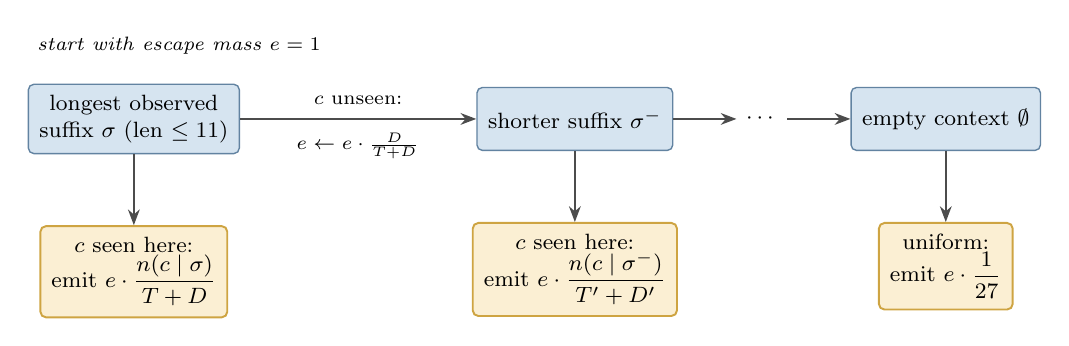
\begin{tikzpicture}[node distance=9mm and 30mm]
  \node[basebox] (s0) {longest observed\\suffix $\sigma$\ (len $\le 11$)};
  \node[basebox,right=of s0] (s1) {shorter suffix $\sigma^{-}$};
  \node[right=8mm of s1,font=\footnotesize] (dots) {$\cdots$};
  \node[basebox,right=8mm of dots] (s2) {empty context $\emptyset$};
  \node[addbox,below=of s0] (e0) {$c$ seen here:\\emit $e\cdot\dfrac{n(c\mid\sigma)}{T+D}$};
  \node[addbox,below=of s1] (e1) {$c$ seen here:\\emit $e\cdot\dfrac{n(c\mid\sigma^{-})}{T'+D'}$};
  \node[addbox,below=of s2] (e2) {uniform:\\emit $e\cdot\dfrac{1}{27}$};
  \draw[flow] (s0)--node[above=0.5mm,midway,font=\scriptsize]{$c$ unseen:}
                    node[below=0.5mm,midway,font=\scriptsize]{$e \leftarrow e\cdot\frac{D}{T+D}$}(s1);
  \draw[flow] (s1)--(dots);
  \draw[flow] (dots)--(s2);
  \draw[flow] (s0)--(e0);
  \draw[flow] (s1)--(e1);
  \draw[flow] (s2)--(e2);
  \node[above=2.5mm of s0.north west,anchor=south west,font=\scriptsize\itshape]
    {start with escape mass $e=1$};
\end{tikzpicture}
\caption{One PPM-C conditional-probability query, $p(c\mid\sigma)$. A single order-12 count table
supplies every context length; the walk moves right only when $c$ is unseen after the current
suffix, multiplying the accumulated escape mass $e$ by $D/(T{+}D)$, and terminates the first time
$c$ has been seen (or at the uniform distribution). Backoff depth is chosen per character, never
fixed globally.}
\label{fig:ppm-flow}
\end{figure}

\paragraph{Provenance.} The initial frozen recipe trained three separate character $n$-grams
(orders 6, 10, and 12) and selected rows from their combined scores. An OOF-only ablation showed the
three fixed-order scores were a redundant view of the same count hierarchy, and the released
recipe replaces them with the single PPM-C-scored table above. The change was made after the
initial freeze using OOF evidence only.

\subsection{Candidate generation: beam search over the lattice}
Candidate rows are proposed by beam search over $L$. A prefix ending at position $i$ is extended
by each of the top-8 characters of position $i{+}1$ (char-top-k~8) and scored as
\[
  \mathrm{score}(t_{1..i+1}) \;=\; \mathrm{score}(t_{1..i}) \;+\; L_{i+1,\,c}
  \;+\; w \cdot \log p_{\mathrm{LM}}(c \mid t_{1..i}),
\]
keeping the best 256 prefixes per position (beam 256), with $\log p_{\mathrm{LM}}$ the PPM-C
conditional score. The search runs twice --- once purely visually ($w{=}0$) and once with the
PPM-C score added ($w{=}1$) --- and the two candidate sets are pooled and deduplicated. Because
the beam emits exactly one character per lattice position, every candidate has the row's length;
the pool differs only in \emph{which} character each position claims. A typical row yields up to a
few hundred distinct candidates.

\subsection{One-parameter row selection}
\label{sec:ranker}
Each pooled candidate $t$ is scored against the \emph{full} (untruncated) lattice with exactly two
quantities:
\[
  \texttt{visual\_sum}(t) = \sum_i L_{i,\,t_i}, \qquad
  \texttt{ppm\_sum}(t) = \sum_i \log p_{\mathrm{PPM}}(t_i \mid t_{<i}).
\]
The second quantity is the same PPM-C score used during proposal generation. Selection is the
transparent interpolation
\[
  S_\lambda(t) = \texttt{visual\_sum}(t) + \lambda\,\texttt{ppm\_sum}(t),
\]
and the candidate with the largest score wins. The interpolation weight $\lambda$ is the layer's
only tuned parameter: a linear grid $\lambda\in[0,4]$ at increments of 0.01 is evaluated directly
on corpus \cer{}, and equal-\cer{} ties choose the smaller language weight.

Selector quality is evaluated with nested fold-heldout tuning: choose $\lambda$ on four clean OOF
folds, then evaluate it on the fifth. All five outer fits select $\lambda=0.84$. After that check,
the same search over all OOF rows also selects $\lambda=0.84$, which is frozen for production.
The candidate table also
yields a \emph{candidate-pool oracle} reference (using the ground truth to pick the lowest-error
retained candidate), which bounds how much any selector could still gain from that finite pool.

\subsection{The decode recipe, end to end}
\label{sec:recipe}
At inference on a new squeeze, the pipeline runs:
\begin{enumerate}
  \item build one dual-light tile1 crop per annotated letter box (R = \texttt{Rotation1},
        G = registered \texttt{Rotation2}, B = \texttt{min(R,G)});
  \item run the all-train \charpost{} classifier with five-view TTA; cache averaged logits;
  \item log-softmax the row's logits into the lattice $L$;
  \item propose candidates: one purely visual beam and one PPM-C-scored beam ($w{=}1$), beam 256,
        char-top-k 8; pool and deduplicate;
  \item compute \texttt{visual\_sum} and \texttt{ppm\_sum} for every candidate against the full lattice;
  \item score with $S_{0.84}$ and select the argmax row;
  \item concatenate selected rows in row order into the squeeze transcript.
\end{enumerate}
After OOF tuning is complete, the all-train \charpost{} classifier and train-only LM produce the
validation, internal-test, and production decodes with exactly this recipe.

\FloatBarrier
\section{The Mechanism on One Real Row}
\label{sec:worked}
Figure~\ref{fig:lattice} shows the whole decision on a single real
internal-test row, picked automatically by the notebook: it scans the cached production decode for
a row where the selector overturns the visual-only argmax \emph{and} lands on the ground truth ---
exactly the situation the layer exists to handle.

The row reads \texttt{TATONANDRAKAIFI}. The visual lattice is confident everywhere except
position~10, where a worn stroke produces a near-tie: the classifier slightly prefers \texttt{N}
($-0.5$ log-prob) over \texttt{K} ($-1.1$). The visual-only argmax therefore reads
\texttt{TATONANDRA\textbf{N}AIFI}, and its total visual score beats the correct row by about
$0.6$ nats --- a margin well inside what stone wear routinely produces. The language model sees
the same choice very differently: after the context \texttt{...TATONANDRA}, the order-12 PPM-C
score prefers the correct continuation by more than $7$ nats
(\texttt{ppm\_sum} $-35.4$ against $-42.7$), because the resulting letter sequence
\texttt{...ANDRA\,KAI...} --- in the underlying Greek, \mbox{AN$\Delta$PA KAI},
``\ldots the man and\ldots'' --- restores \emph{kai}, the most common conjunction in the
language, where the visual read leaves a non-word. With the OOF-tuned $\lambda=0.84$, the selector
accepts the small visual deficit in exchange for the large language gain and selects the true row.

This is the intended division of labor, visible end to end: visual evidence proposes and
constrains; language evidence arbitrates near-ties; one OOF-tuned scalar decides how much it is
worth relative to the lattice.

\IfFileExists{figs/charpost_lattice_graph.png}{%
\begin{figure}[!htbp]
  \centering
  \maybeinclude[width=0.75\textwidth]{figs/charpost_lattice_graph.png}
  \caption{The \charpost{} row lattice for the worked example. Boxes are per-position character
  posteriors with log probabilities (top four shown, plus any read-out letter outside them); faint
  lines are the beam's transitions. Dashed: visual-only argmax; solid: selector-selected row; ground
  truth is drawn separately only when it differs from the selector's choice. Long rows are windowed
  around the disagreement.}
  \label{fig:lattice}
\end{figure}}{}

\section{Results}
\label{sec:results}
Table~\ref{tab:results} records the \model{} line-model reference numbers, the
\charpost{} results on the internal validation and test splits, and the external production
result. The line-model rows use the plain TrOCR decoder, which is \emph{not} part of the deployed
decode path (Section~\ref{sec:duallight}); they are a diagnostic for the visual backbone, not a
baseline the deployed system regresses from. On the same internal splits, the full pipeline cuts
the line model's \cer{} from 0.0358 to 0.0229 on validation and from 0.0320 to 0.0222 on test ---
31--36\% relative error reduction.

\begin{table}[htbp]
\centering
\small
\caption{Recorded metrics. Lower \cer{} is better. The three official v2 rows grade the same
released decode with the verbatim contest scorer; their character totals are not per-row
comparable to the internal \cer{} (Section~\ref{sec:protocol}).}
\label{tab:results}
\begin{tabular}{@{}llll@{}}
\toprule
\textbf{Artifact / run} & \textbf{Split} & \textbf{Setting} & \textbf{\cer{} $\downarrow$} \\
\midrule
\model{} line reference & internal validation & train-only LM & 0.0358 \\
\model{} line reference & internal test & train-only LM & 0.0320 \\
\model{} line reference & internal test & train+validation LM & 0.0310 \\
\charpost{} ($\lambda=0.84$) & internal validation & one-parameter selector & 0.0229 \\
\charpost{} ($\lambda=0.84$) & internal test & one-parameter selector & 0.0222 \\
\charpost{} ($\lambda=0.84$) & \texttt{trogs26-test-ppm} & internal CER (per-row) & \textbf{0.0838} \\
\charpost{} ($\lambda=0.84$) & \texttt{trogs26-test-ppm} & official v2 \texttt{all\_cer} & 0.0786 \\
\charpost{} ($\lambda=0.84$) & \texttt{trogs26-test-ppm} & official v2 \texttt{opt\_cer} & 0.0801 \\
\charpost{} ($\lambda=0.84$) & \texttt{trogs26-test-ppm} & official v2 \texttt{cer} (confident) & 0.1166 \\
\bottomrule
\end{tabular}
\end{table}

Validation and internal test are report-only after the recipe freeze: they were not used to
choose the selector, which is selected by the nested OOF comparison below.

\paragraph{What the selector contributes.} Figure~\ref{fig:ladder} is deliberately restricted to
recipe-consistent OOF evidence. The visual-only argmax scores \cer{} 0.0855; the fold-heldout
one-parameter selector scores 0.0498; the ground-truth-selected candidate-pool oracle scores
0.0125. The selector therefore removes about 49\% of the errors separating visual-only decoding from
the candidate-pool bound. This oracle is a retrieval diagnostic, not an attainable performance
claim: it chooses only among the finite candidates retained by the beam, but uses the ground truth
to do so. It shows that most remaining OOF errors are \emph{selection} errors, not retrieval
errors: the right answer is usually already in the pool.

\IfFileExists{figs/charpost_cer_ladder.png}{%
\begin{figure}[htbp]
  \centering
  \maybeinclude[width=0.68\linewidth]{figs/charpost_cer_ladder.png}
  \caption{Recipe-consistent OOF decode ladder: visual-only argmax, the nested fold-heldout
  one-parameter selector, and the ground-truth-selected candidate-pool oracle.}
  \label{fig:ladder}
\end{figure}}{}

\FloatBarrier
\section{Reproducibility}
The notebook \texttt{greek\_squeezes.ipynb} validates or rebuilds the artifact tree under
\texttt{data/} and regenerates the report figures and companion diagnostics into
\texttt{report/figs/} from cached artifacts --- the lattice graph (including automatic selection
of the worked-example row), its full-alphabet heatmap companion, the confusion matrix, the CER
ladder, the selector tuning curve, and the model-view figures. The same pipeline runs on Modal:
\texttt{modal\_app.py} builds all artifacts from scratch and stages production decodes under
\texttt{data/prod\_runs/}, and \texttt{modal\_notebook.py} executes the notebook end to end
against the prepared volume and persists the regenerated figures. Reusable artifacts are shared
through the project Hugging Face bucket, \texttt{hf://buckets/papadimas/greek\_squeezes}.

\section{Conclusion}
Reading squeezes well required respecting what a squeeze physically is. The dual-light packing
lets one encoder read both raking-light views --- and their dark-stroke union --- in a single
pass; the \charpost{} layer then re-derives the transcript through an explicit lattice in which
visual and language evidence are separately visible and their single relative weight is tuned on
clean out-of-fold data. The one-parameter selector cuts the line model's internal \cer{} by
31--36\% (to 0.0229 on validation and 0.0222 on test). The released selector scores
\cer{} 0.0838 on 50 genuinely unseen squeezes (official v2 \texttt{all\_cer} 0.0786 on the
same decode); the external set was not used to tune the selector. The system can
show its work: for any row it can display the lattice, the candidates,
and the exact scores that decided the output. The full system is reproducible from
\texttt{greek\_squeezes.ipynb}, cacheable under \texttt{data/}, and runnable on Modal.

\begin{thebibliography}{9}\footnotesize
\bibitem{howe2025} Howe, N.R., Chang, F., Falbo, I., Brown, T. \& Hershkowitz, A.
  \textit{Character Recognition for Greek Squeezes.} IJDAR \textbf{28}, 345--356 (2025).
\bibitem{li2023} Li, M.\ et al.\ \textit{TrOCR: Transformer-based Optical Character Recognition
  with Pre-trained Models.} Proceedings of the AAAI Conference on Artificial Intelligence
  \textbf{37}(11), 13094--13102 (2023). arXiv:2109.10282.
\bibitem{cleary1984} Cleary, J.G. \& Witten, I.H. \textit{Data Compression Using Adaptive Coding
  and Partial String Matching.} IEEE Transactions on Communications \textbf{32}(4), 396--402
  (1984).
\bibitem{bell1990} Bell, T.C., Cleary, J.G. \& Witten, I.H. \textit{Text Compression.}
  Prentice Hall (1990).
\bibitem{moffat1990} Moffat, A. \textit{Implementing the PPM Data Compression Scheme.}
  IEEE Transactions on Communications \textbf{38}(11), 1917--1921 (1990).
\end{thebibliography}
{\footnotesize\noindent The implementation uses PyTorch, Hugging Face \texttt{transformers},
OpenCV, and scikit-learn. Section~\ref{sec:protocol} defines the exact \cer{} convention used for
every number in this report.}

\end{document}
